
\documentclass[11pt ,A4]{article}
% \usepackage{amsmath} % \usepackage is a command that allows you to add functionality to your LaTeX code
\usepackage[a4paper, total={7in, 9in}]{geometry}
% \usepackage[sfdefault]{roboto}

\usepackage[none]{hyphenat}
% \usepackage{url}
\usepackage[colorlinks=true, allcolors=blue]{hyperref}
\usepackage{indentfirst}

\usepackage{graphicx}
\graphicspath{ {./images/} }

\usepackage{float}

\setlength{\parindent}{0.5cm}

\title{Jocului Vieții\\Proiectul 6}
\author{Capisizu Cosmin Louis\\IS1.1} % Sets authors name
% \date{\today}

\begin{document}
    \maketitle % creates title using information in preamble (title, author, date)
    \pagebreak

    \section{Cerința} % creates a section
        \paragraph{}
            Proiectarea si implementarea unui sistem multi-agent pentru simularea jocului vieții, game of life. Se va defini si analiza cel puțin un joc de tip automat celular diferit de cel din programul demonstrativ pentru jocul vieții. Pentru jocul vieții se vor defini si experimenta si alte configurații inițiale, pe lângă cele predefinite in programul demonstrativ.

    \section{Prezentarea jocului}

        \paragraph{}Jocul Vieții, cunoscut si sub numele de Viata, este un automat celular conceput de matematicianul britanic John Horton Conway in 1970. Este un joc fără jucători, ceea ce înseamna ca evoluția sa este determinata de starea sa inițiala, nefiind nevoie de alte informații.

        \paragraph{} Se interacționează cu Jocul Vieții creând o configurație inițială si observând cum evoluează. Este Turing complet si poate simula un constructor universal sau orice alta mașina Turing.

        \paragraph{} Universul Jocului Vieții este o rețea ortogonala infinita, bidimensionala, de celule pătrate, fiecare dintre acestea fiind într-una dintre cele doua stări posibile, vie sau moarta (sau populata si, respectiv, nepopulata). Fiecare celula interacționează cu cei opt vecini ai sai, care sunt celulele care sunt adiacente orizontal, vertical sau diagonal.

        \paragraph{} La fiecare pas in timp, au loc următoarele tranziții
        \begin{itemize}
            \item Orice celula vie cu mai puțin de doi vecini vii moare, ca prin subpopulare.
            \item Orice celula vie cu doi sau trei vecini vii trăiește in generația următoare.
            \item Orice celula vie cu mai mult de trei vecini vii moare, ca prin suprapopulare.
            \item Orice celula moarta cu exact trei vecini vii devine o celula vie, ca prin reproducere.
        \end{itemize}

        \paragraph{} La fiecare pas in timp, au loc următoarele tranzitii Aceste reguli, care compara comportamentul automatului cu viata reala, pot fi condensate in următoarele
        \begin{itemize}
            \item Orice celula vie cu doi sau trei vecini vii supraviețuiește.
            \item Orice celula moarta cu trei vecini vii devine o celula vie.
        \end{itemize}

        \paragraph{} Toate celelalte celule vii mor in generația următoare. In mod similar, toate celelalte celule moarte rămân moarte.

        \paragraph{} Modelul inițial constituie sămânța sistemului. Prima generație este creata prin aplicarea regulilor de mai sus simultan la fiecare celula din sămânță, vie sau moarta; nașterile si decesele au loc simultan, iar momentul discret in care se întâmpla acest lucru se numește uneori căpușa. Fiecare generație este o funcție pura a celei precedente. Regulile continua sa fie aplicate in mod repetat pentru a crea generații viitoare.

    \section{Problema studiata}

        \paragraph{}
        In cadrul acestui proiect, problema consta in implementarea si stimularea agenților din cadrul jocului vieții.
        Acesta probleme are mai multe cerințe: Simularea sistemului multi-agent, analiza comportamentului agenților, si crearea unei modalități de alterare a parametrilor simulării.
        

    \section{Metoda de rezolvare folosita}

        \paragraph{}
            Pentru implementarea sistemului, analiza datelor dar si alterarea parametrilor simulării s-lau folosit mai multiple tehnologii web.

            Fundația aplicației este construita folosind framework-ul "React" construit de "Facebook", dar si alte tehnologii cum ar fi "TypeScript" si "Sass".

        \subsection{Sistemul multi-agent}
            \paragraph{}
                Acest sistem a fost construi folosind o clasa ce incorporează funcționalitatea dar si datele necesare simulării.
                Ca si structura de date ce stochează starea simulării s-a folosit matricea. Aceasta oferă un acces simplu si rapid asupra stării agenților. 

        \subsection{Parametri simulării}
            \paragraph{}
                Pentru a permite utilizatorului sa interacționeze cu sistemul multi-agent s-au implementat următoarele funcționalități: modificarea manuala a stării unei celule folosind mouseul, modificarea dimensiunii simulării folosind interfața grafica si modificarea si resetarea regulilor folosind editorul din simulare.  
            
        \subsection{Implementarea simulării}
            \paragraph{}
                \textbf{O celula} poate fi vie sau morta, aceste stări fiind reprezentate de 1 sau 0 logic.
                Tabloul ce este format din mulțimea celulelor este stocat într-o matrice. Aceasta structura este implementata la rândul ei ca fiind un vector de vectorii de stări logice. 
                \begin{figure}[H]
                    \centering
                    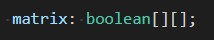
\includegraphics[scale=0.8]{matrix_matrix_def}
                    \caption{Declararea matricii}
                \end{figure}

            \paragraph{}
                \textbf{Starea celulelor} este modificata de către clasa din care fac parte, astfel celula in sine are doar funcționalitatea de a-si retine propria stare.

            \paragraph{}
                \textbf{Regulile de evoluție} sunt oferite de către un obiect ce deține o listă de reguli.
                Acest obiect este inițializat folosind setul de reguli de baza. Obiectul conține o listă de cerințe.
                Fiecare cerința are la rândul ei o lista de intervale si un set de condiții logice.
                Aceste condiții sunt folosite pentru a determina daca un anumit scenariu se aplica.
                In cazul in care scenariul est confirmat ca fiind potrivit pentru starea actuala se folosește un alt set intern de condiții ce stabilesc starea următoare a celulei.
            
            \paragraph{}
                \textbf{Evoluția celulelor} este realizata de o metoda a clasei.
                Aceasta funcție analizează datele ce sunt prezente in generația actuala si folosește instrucțiunile oferite de către serul de reguli pentru a genera următoare generație.

            \paragraph{}
                \textbf{Dimensiunea simulării} este predefinita dar se poate mari sau micșora folosind interfața grafica.
                Modificarea simulării nu duce la pierderea stării, excepție de la aceasta regula o face micșorarea simulării astfel încât celulele depășesc limita acesteia.
                Atât mărirea cat si micșorarea se face începând in coltul cel mai îndepărtat fata de origine.

        \subsection{Implementarea interfeței grafice}
            \paragraph{}
                Acest sistem pune accent pe implementarea modelului multi-agent, astfel interfața comanda si afișează starea simulării.
                Astfel arhitectura necesara implementării interfeței nu afectează sistemul simulat.

            \paragraph{}
                \textbf{Compatibilitatea dintre sistem si interfața grafica} se face folosind interfețele.
                Sistemul multi-agent implementează o interfața ce permite interfeței grafice sa acceseze resursele necesare acesteia.
                \begin{figure}[H]
                    \centering
                    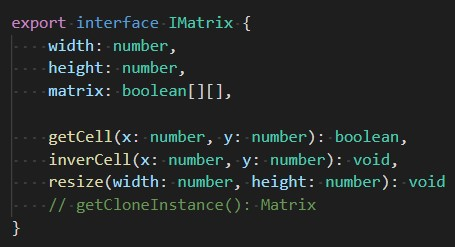
\includegraphics[scale=0.8]{IMatrix_interface}
                    \caption{Interfața implementata de matrice}
                \end{figure}

                De asemenea interfața grafica are mai multe implementări ce implementează si ele la rândul lor o interfață.



            \paragraph{}
                \textbf{Interfața grafica} este implementata folosind doua sisteme diferita: componente web native si implementarea grafica folosind o librărie grafica specializata.
                Acestea doua implementări sunt abstractizate si pot fi interschimbate  in timp real de către utilizator.
                \begin{figure}[H]
                    \centering
                    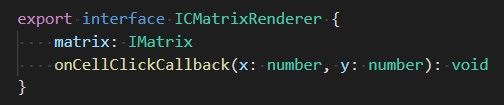
\includegraphics[scale=0.8]{ICMatricRenderer_interface}
                    \caption{Interfața implementata de sistemele de randare}
                \end{figure}

    \section{Funcționarea programului pentru experimentare}

        \paragraph{}
            O caracteristică esențială in cardul unei simulări este posibilitatea de a interacționa cu acel mediu si de a-i modifica parametri.
            Sistemul multi-agent implementat prezintă un număr mare de parametri si opțiuni ce pot fi schimbate in timp real.
            Parametrii inițiali sunt prestabiliți dar pot fi oricând modificați in carul simulării.

            Parametrii ce pot fi modificați folosind interfața grafica pot altera: dimensiunea sistemului, regulile de evoluție si interacțiunea directa cu un agent.
        
        \paragraph{}
            \textbf{Interactiunea cu starea sistemului} se poate face folosind mausul sau butoanele din cardul interfeței grafice sau tastatura.

        \paragraph{}
            \textbf{Mijloacele de interacțiune directa:}
            \begin{itemize}

                \item 
                    \textbf{Mausul} permite schimbarea directa a stării cărei celule.
                    Culoarea celulei selectate se schimba pentru a evidenția selecția acesteia.

                \item 
                    \textbf{Tastatura} permite resetarea sau incrementarea generației simulării.
                    Folosind tasta "space" se poate trece la generația următoare.
                    Pentru a simula cu rapiditate aceasta tasta se poate tine apăsata.
                    Combinația de taste "ctrl" si "r" comanda setarea la starea inițială a sistemului.

                \item
                    \textbf{Editorul de reguli} permite utilizatorului sa modifice regulile de evoluție ale sistemului in timp real.
                    Acesta integrare este foarte importanta in cadrul acestui proiect întrucât permite analiza sistemului in funcție de regulile impuse.
                    Starea inițială a regulilor este cea prezentata in cadrul prezentării jocului.

            \end{itemize}
            
            \begin{figure}[H]
                \centering
                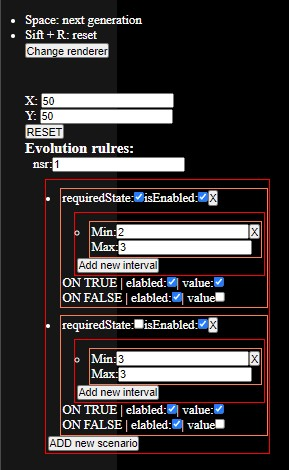
\includegraphics[scale=1]{setings}
                \caption{Parametrii disponibili utilizatorului}
            \end{figure}

            
        \paragraph{}
            \textbf{Dimensiunea sistemului} este prezentata sub forma a doua numere ce reprezinta numărul de linii si de coloane.
            Simularea începe inițial având o dimensiune de 50 pe 50 de celule.
            Acest număr o fost ales deoarece perforează simularea in timp real.
            Maximul impus prin cod este de 500 pe 500 de celule, punct in care simularea încă se mișcă decent dar solicita deja destul de multe resurse.
            Schimbarea acestor valori nu distruge stare curenta a agenților decât daca aceștia ies din spațiul de simulare.
            La introducerea spațiului nou celulele sunt inițializate ca fiind inactive.

        

    \section{Cazuri experimentale}
        \paragraph{}
            Principalele cazuri experimentale in cardul acestui sistem sunt formațiile celulare ce pot fi create.
            Aceste organisme sunt de mai multe tipuri si au diferite stări.

            Cele mai întâlnite formații sunt nave spațiale si organismele multi stabile.
            Navele spațiale pot fi formate dintr-un număr mic sau mare de celule.
            Organismele stabile pot avea de la os tare pana la N stări.

            \subsection{Nave spațiale}
                \begin{itemize}

                    \item \textbf{Planor} acest organism are 4 stări si se mișca pe diagonala.
                        \begin{figure}[H]
                            \newcommand\lp{organisme/nave/planor}
                            \centering
                            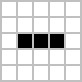
\includegraphics[scale=0.8]{\lp/1}
                            
\includegraphics[scale=0.8]{\lp/2}
                            
\includegraphics[scale=0.8]{\lp/3}
                            
\includegraphics[scale=0.8]{\lp/4}
                            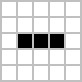
\includegraphics[scale=0.8]{\lp/1}
                            \caption{Cele 4 stari are planorului}
                        \end{figure}

                    \item \textbf{Navă spațială mica} are tot 4 si se mișca pe axa verticala si orizontala.
                          Celelalte nave spatiale au același comportament dar difer prin dimensiune.
                        \begin{figure}[H]
                            \newcommand\lp{organisme/nave/navaMica}
                            \centering
                            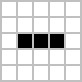
\includegraphics[scale=0.7]{\lp/1}
                            
\includegraphics[scale=0.7]{\lp/2}
                            
\includegraphics[scale=0.7]{\lp/3}
                            
\includegraphics[scale=0.7]{\lp/4}
                            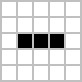
\includegraphics[scale=0.7]{\lp/1}
                            \caption{Cele 4 stări are navei spatiale mici}
                        \end{figure}

                    \item Navă spațială medie
                        \begin{figure}[H]
                            \centering
                            
\includegraphics[scale=0.7]{organisme/nave/navaMedie}
                            \caption{Nava spatiala medie}
                        \end{figure}

                    \item Navă spațială mare
                        \begin{figure}[H]
                            \centering
                            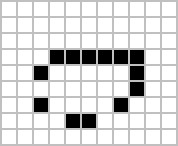
\includegraphics[scale=0.7]{organisme/nave/navaMare}
                            \caption{Nava spatiala mare}
                        \end{figure}

                \end{itemize}
                
            \subsection{Organisme stabile}

                \paragraph{}
                    Aceste organisme mențin o forma stabila formata din una sau mai multe stări.
                    Deși forma este stabila interacțiunea cu alte organisme o poate destabiliza.
                    \begin{figure}[H]

                        \newcommand\lp{organisme/stabile}
                        \newcommand\locIngScale{0.8}
                        \newcommand\locTextScale{0.33}

                        \begin{figure}[H]
                            \begin{minipage}{\locTextScale\textwidth}
                            \centering
                            
\includegraphics[scale=1]{\lp/1-bloc}
                            \caption{Bloc}
                            \end{minipage}\hfill
                            % 
                            \begin{minipage}{\locTextScale\textwidth}
                            \centering
                            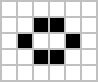
\includegraphics[scale=\locIngScale]{\lp/2-stup}
                            \caption{Stup}
                            \end{minipage}
                            % 
                            \begin{minipage}{\locTextScale\textwidth}
                            \centering
                            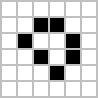
\includegraphics[scale=0.7]{\lp/3-felie}
                            \caption{Felie}
                            \end{minipage}
                        \end{figure}

                        \begin{figure}[H]
                            \begin{minipage}{\locTextScale\textwidth}
                            \centering
                            
\includegraphics[scale=\locIngScale]{\lp/4-barca}
                            \caption{Barca}
                            \end{minipage}
                            % 
                            \begin{minipage}{\locTextScale\textwidth}
                            \centering
                            
\includegraphics[scale=\locIngScale]{\lp/5-tub}
                            \caption{Tub}
                            \end{minipage}
                        \end{figure}
                    \end{figure}
                       
            \subsection{Organisme multistabile}
                    
                    \paragraph{}
                        Aceste organisme oscilează intre mai multe stări stabile.
                        Sistemul celular format de către aceste se poate deregla doar prin interacțiune cu alte organisme.

                    \begin{figure}[H]
                        \newcommand\lp{organisme/oscilante/1-blinker}
                        \centering
                        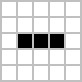
\includegraphics[scale=0.7]{\lp/1}
                        
\includegraphics[scale=0.7]{\lp/2}
                        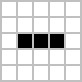
\includegraphics[scale=0.7]{\lp/1}
                        \caption{Blinker}
                    \end{figure}

                    \begin{figure}[H]
                        \newcommand\lp{organisme/oscilante/2-toad}
                        \centering
                        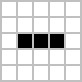
\includegraphics[scale=0.7]{\lp/1}
                        
\includegraphics[scale=0.7]{\lp/2}
                        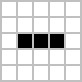
\includegraphics[scale=0.7]{\lp/1}
                        \caption{Toad}
                    \end{figure}
                    
                    \begin{figure}[H]
                        \newcommand\lp{organisme/oscilante/3-beacon}
                        \centering
                        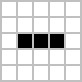
\includegraphics[scale=0.7]{\lp/1}
                        
\includegraphics[scale=0.7]{\lp/2}
                        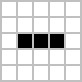
\includegraphics[scale=0.7]{\lp/1}
                        \caption{Beacon}
                    \end{figure}
                    
                    \begin{figure}[H]
                        \newcommand\lp{organisme/oscilante/4-pulsar}
                        \centering
                        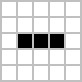
\includegraphics[scale=0.8]{\lp/1}
                        
\includegraphics[scale=0.8]{\lp/2}
                        
\includegraphics[scale=0.8]{\lp/3}
                        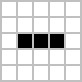
\includegraphics[scale=0.8]{\lp/1}
                        \caption{Pulsar}
                    \end{figure}

                    \begin{figure}[H]
                        \newcommand\lp{organisme/oscilante/5-pentadecathlon}
                        \centering
                        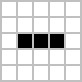
\includegraphics[scale=0.8]{\lp/1}
                        
\includegraphics[scale=0.8]{\lp/2}
                        
\includegraphics[scale=0.8]{\lp/3}
                        
\includegraphics[scale=0.8]{\lp/4}
                        
\includegraphics[scale=0.8]{\lp/5}
                        
\includegraphics[scale=0.8]{\lp/6}
                        
\includegraphics[scale=0.8]{\lp/7}
                        
\includegraphics[scale=0.8]{\lp/8}
                        
\includegraphics[scale=0.8]{\lp/9}
                        
\includegraphics[scale=0.8]{\lp/10}
                        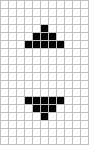
\includegraphics[scale=0.8]{\lp/11}
                        
\includegraphics[scale=0.8]{\lp/12}
                        
\includegraphics[scale=0.8]{\lp/13}
                        
\includegraphics[scale=0.8]{\lp/14}
                        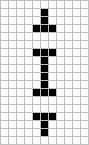
\includegraphics[scale=0.8]{\lp/15}
                        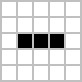
\includegraphics[scale=0.8]{\lp/1}
                        
                        \caption{Pulsar}
                    \end{figure}

                


    \section{Probleme întâlnite}
        \paragraph{} 
            Simulările multi-agent prezintă multe obstacole si probleme.
            Principalele dificultăți in cadrul acestui proiect sunt:
        \begin{itemize}
            \item Implementarea sistemului ce retine si modifica starea agenților.
                Acest sistem poate fi implementat folosind diferite structuri de date, cum ar fi: matricile sau listele.
                Principalul avantaj al matricii este accesul direct al oricărui agent dar si al vecinilor acestuia, un mare dezavantaj este faptul ca odată cu creșterea dimensiunii sumulării creste si mărimea matricii.
                Simularea folosind liste permite o scalare mai ușoara si o separare dintre numărul total de agenți posibil si mărimea mediului de simulare.
                Cel mai mare dezavantaj consta in faptul ca anumite operații sunt mult mai greu de implementat si necesita mult mai mulți pași de execuție.
                In cazu acestui proiect matricea a fost folosita ca si mijloc de stocare al datelor.
            \item Implementarea si unei interfețe grafice ce permite interacțiunea directa cu simularea.
                Interfața grafica si simularea necesita arhitecturi total diferite.
                Deci simularea sistemului este punctul de referință, interfața grafica afișează si modifica datele la cererea utilizatorului.
        \end{itemize}

    % 8 
    \section{Modificările si îmbunătățirile necesare}
        \paragraph{}
            Deși modelul de baza este implementat se pot adaugă multe funcționalități.
            Simularea acestei probleme se poate face cu un număr foarte mare de parametrii si condiții. 

            Multe componente deja implementate necesita anumite funcționalități pentru a opera mult mai satisfăcător.
            De asemenea parte de organisme ce pot fi create se poate implementa folosind o lista predefinita.

            \subsection{Modificări necesare}
                Din punct de vedere tehnic sunt necesare urmatoarele:
                \begin{itemize}
                    \item Optimizarea funcțiilor ce generează datele următoarei generații.
                    \item Implementarea a unei liste ce are rolul de a stoca doar celulele ce sun active.
                          Aceasta structura poate fi folosita pentru eficientizarea procesului se afișare.
                    \item Modificări asupra sistemelor de randare.
                \end{itemize}


            \subsection{Potențiale îmbunătățiri}
                
                \begin{itemize}
                    \item Posibilitatea de a alege organisme ce pot fi simulate din cadrul unei liste.
                    \item Implementarea unui sistem mai bun de randare.
                    \item Implementarea unui sistem mai bun de reguli.
                    \item Implementarea unui sistem de analiza a datelor simulării.
                    \item Opțiunea de a salva starea curenta.
                    \item Posibilitatea de a întoarce sistemul într-o stare anterioara.
                \end{itemize}
                
             
    \section{Referințe}

        \begin{itemize}
            \item \href{https://en.wikipedia.org/wiki/Conway%27s_Game_of_Life}{wiki | Conway's Game of Life}
        \end{itemize}


\end{document} 